\documentclass{article}
\usepackage[utf8]{inputenc}

\title{Rapport psc}
\author{groupe info}

\usepackage{natbib}
\usepackage{graphicx}

\begin{document}

\maketitle

\section{Introduction}

sur vrep

\section{Présentation du programme central}
\subsection{Vue d'ensemble}
Comme précisé dans le rapport intermédiaire, le programme principale a été écrit en python, son rôle est de gérer l'ensemble des entrées pour produire les actions que doit réaliser le robot. Ces entrées sont : l'ensemble des distances envoyés par les capteurs présents sur le robot, les positions des éléments envoyés par la caméra puis le retour de l'Arduino après une tentative de réalisation d'une action donnée (figure \ref{fig:schema}).

\begin{figure}[h!]
\centering
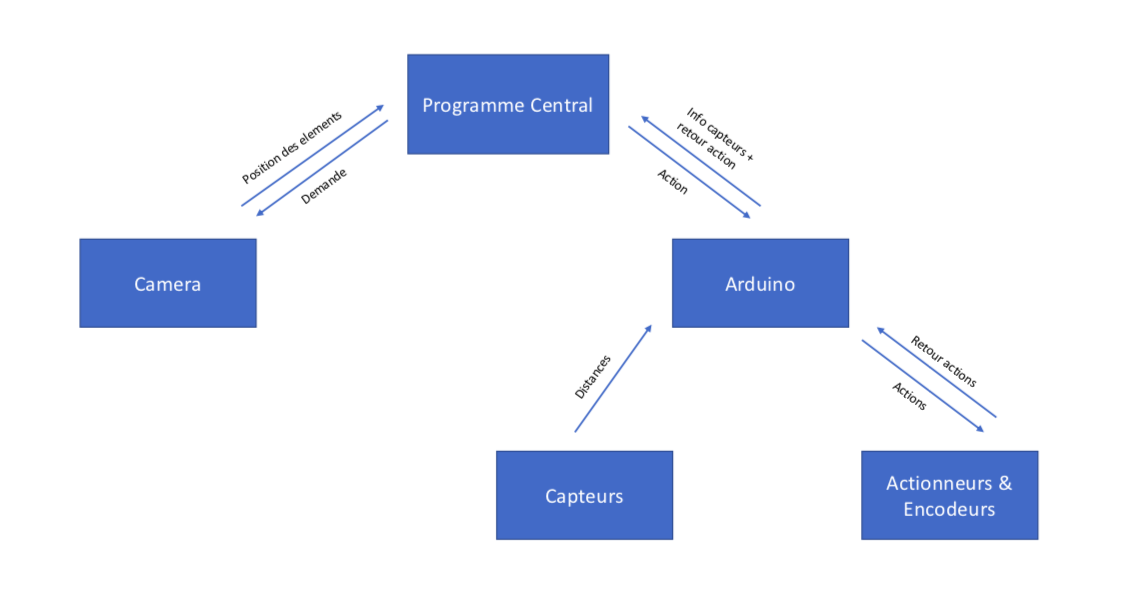
\includegraphics[scale=0.3]{schema}
\caption{Schéma représentatif du fonctionnement du robot}
\label{fig:schema}
\end{figure}


\subsection{Implémentation}

Pour réaliser le schéma précèdent, le code a été conçu comme suit (figure \ref{fig:program}): \\

\begin{figure}[h!]
\centering
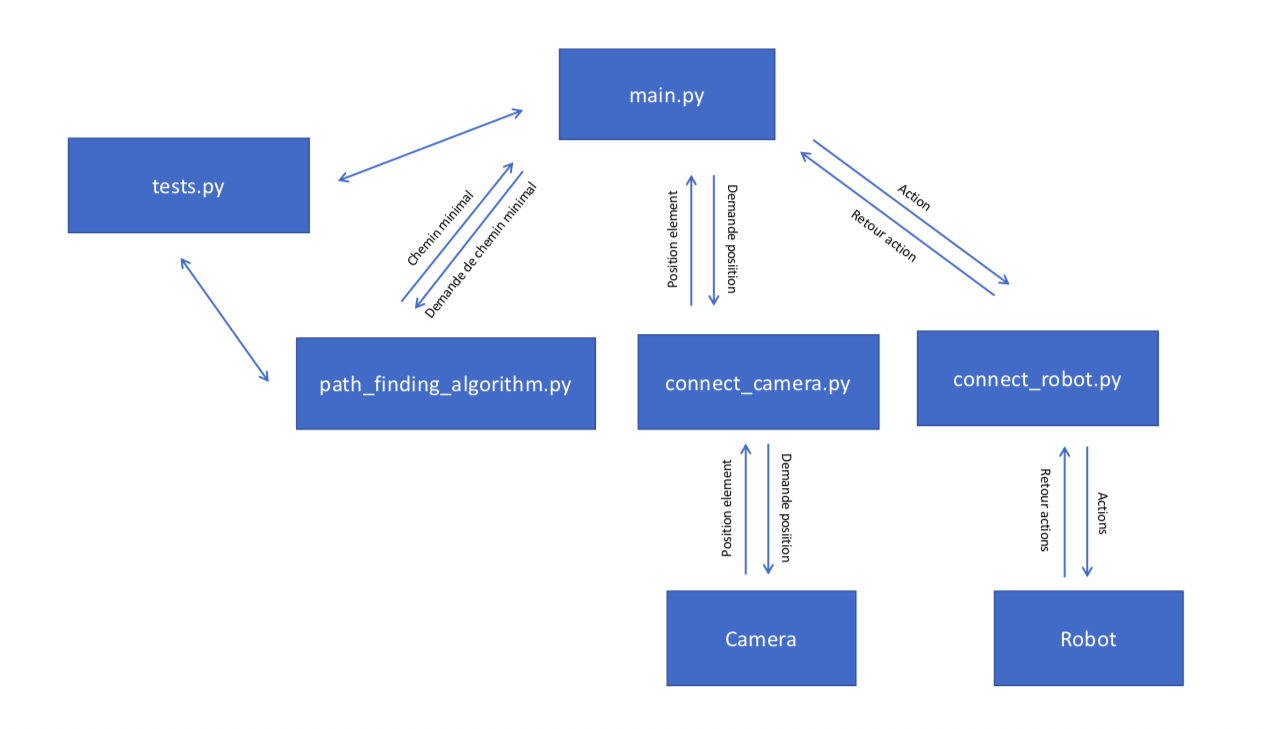
\includegraphics[scale=0.3]{program}
\caption{Représentation schématique du programme}
\label{fig:program}
\end{figure}

{\renewcommand\labelitemi{-}
\begin{itemize}
\itemsep0em
\item \textbf{main.py:} fichier principal qui traite les informations d'entrée et trouve à l'aide d'un algorithme de calcul de chemin (codé indépendamment dans le fichier path\_finding\_algortihm.py) la prochaine étape à faire par l'Arduino, puis en se basant sur le retour de celle-ci ainsi que des retours de la caméra, ce programme fait une mise à jour de ce qui est connu sur la table de jeu pour pouvoir générer à nouveau la prochaine étape à suivre.\\
\item \textbf{connect\_robot.py:} fichier contenant les fonctions qui permettent l'envoie des commandes à l'Arduino et la réception d'un retour.\\
\item \textbf{connect\_camera.py:} contient les fonctions nécessaires à la communication avec la caméra.\\
\item \textbf{path\_finding\_algorithm.py:} contient l'algorithme utilisé pour le calcul des chemins lors du mouvement du robot.\\
\item \textbf{tests.py:} utilisé pour tester l'ensemble des fonctions codés.
\end{itemize}
}

Conformément à ce qu'on avait pris comme convention au début, le retour de l'Arduino est de la forme "$a_{1}a_{2}a_{3}....a_{21}$" où $a_{1} = 0$ si l'action demandée à l'Arduino n'as pas pu être accomplie (robot qui rencontre un obstacle dans son chemin par exemple) et $a_{1} = 1$ dans le cas contraire, puis $a_{2}a_{3}$ , $a_{4}a_{5}$, .. $a_{2i}a_{2i+1}$ .. , $a_{12}a_{13}$ sont des nombres à deux chiffres représentant la distance en centimètres du capteur numéro $i$ pour $a_{2i}a_{2i+1}$ à ce qu'il voit devant lui, finalement $a_{14}..a_{17}$ et  $a_{18}..a_{21}$ représentent respectivement la distance rée le parcourue par le robot et l'angle réel de sa rotation au début de l'action en millimètres.

En ce qui concerne le retour de la caméra, celui ci sera de la forme "$a_{1}a_{2}....a_{243}$" (flux de taille $log_{2}(234) = 7.87 bits$) où chaque 6 chiffres représentent respectivement les cordonnées (x, y) en décimètres d'un élément de la table (il y en a 40 : 37 atome et 3 robots) et les 3 derniers chiffres l'orientation du robot.

\\ \\
Pour rappel, le robot doit réaliser les taches suivantes: \textbf{déplacer les atomes}, \textbf{lancer une expérience}, \textbf{peser des atomes} ou \textbf{libérer un atome}. L'ensemble de ces actions peut être réalisé en utilisant cinq actions élémentaires, à savoir, \textbf{avancer}, \textbf{tourner à droite}, \textbf{tourner à gauche}, \textbf{attraper un élément}, \textbf{poser un élément}. C'est les cinq actions implémentés par l'algorithme.

La table de jeu est de dimensions 2 mètres x 3 mètres, le choix qui a été fait est de la représenter par une matrice de dimensions [$2 \times ratio, 3 \times ratio$] initialisée à des zéros où le $ratio$ est une variable globale à choisir par l'utilisateur qui donne des résolutions différentes (et de là des précisions différentes du mouvement du robot), elle est à choisir selon la puissance de la machine exécutant le programme et les contraintes des cahiers de charge (nous l'avons initialisé à 100 ce qui veut dire une précision de 1cm dans les déplacements du robot) (figure \ref{fig:ratiofig}) 

\begin{figure}[h!]
\centering
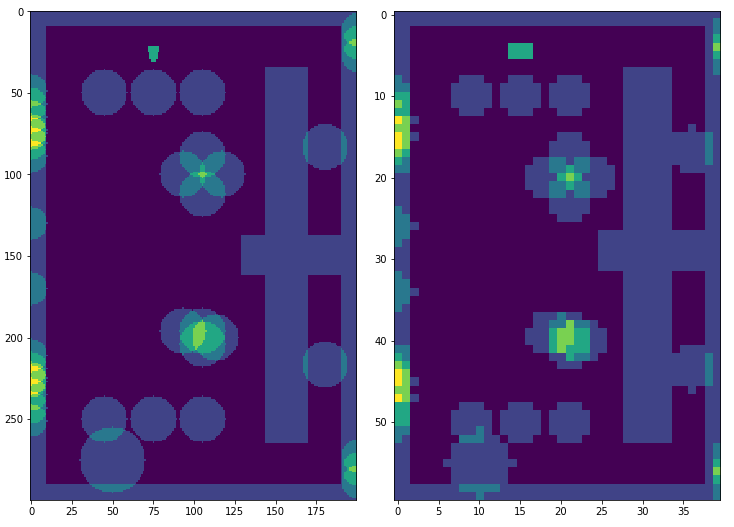
\includegraphics[scale=0.45]{ratiofig}
\caption{Table de jeu dans les deux cas ratio = 100 et ratio = 20}
\label{fig:ratiofig}
\end{figure}

Les différents cercles dans la figure (figure \ref{fig:ratiofig}) représentent les zones interdites au centre du robot (figure \ref{fig:zone}), ainsi deux zones peuvent se superposer si les deux éléments correspondants sont proches à moins du diamètre du robot près. L'ajout d'un élément à la table se fait en augmentant les coefficients de la matrice dans la zone correspondante de 1, cette idée facilitera la suppression d'un élément en baissant simplement les coefficients de cette zone de 1 alors que si des zones superposés ont été représentés comme une seule zone de "uns" dans la matrice, la suppression de l'une d'elle supprimera une partie de l'autre (problème rencontré au début).

\begin{figure}[h!]
\centering
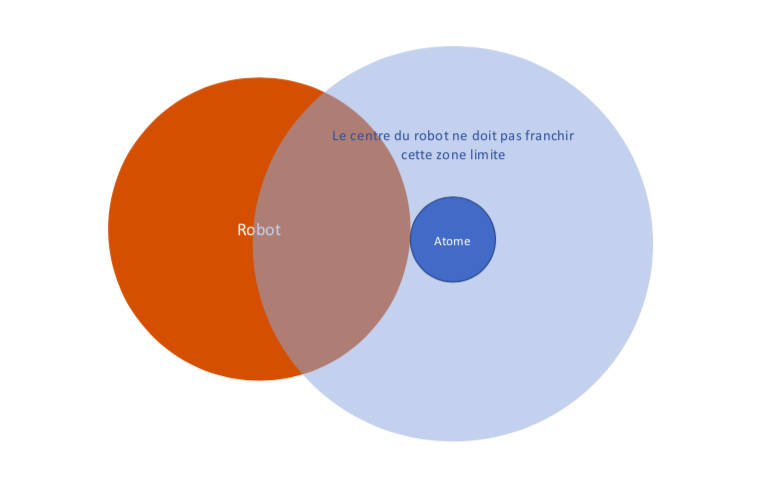
\includegraphics[scale=0.4]{zone}
\caption{Zone interdite au centre du robot}
\label{fig:zone}
\end{figure}

Le centre du robot doit alors se déplacer dans les zones nulles de la matrice pour réaliser les taches voulues.

Les éléments de la table sont représenté par les trois classes d'objets: \textit{robot}, \textit{atom} et \textit{target} (qui est un élément fictif représentant un point de la table). Ces trois classes héritent d'une classe commune \textit{element} vu leurs propriétés communes.

En ce qui concerne l'orientation du robot, celle-ci est repérée à  l'aide de l'angle $\theta \in [-\pi, \pi]$ que fait le devant du robot avec l'axe des abscisses et qui est positif dans la direction des ordonnées positifs. (voir figure  \ref{fig:theta})


Voici la version la plus récente du programme:
\href{https://github.com/Coupe-de-France-de-robotiques/algorithmique/tree/master}

N'hésitez pas à changer les paramètres globales en haut du fichier main.py pour voir les différents effets de ceux-ci et d'utiliser le fichier tests.py pour faire des tests (pour lancer la boucle principale, décommentez la fonction mn.action())
\begin{figure}[!h]
\centering
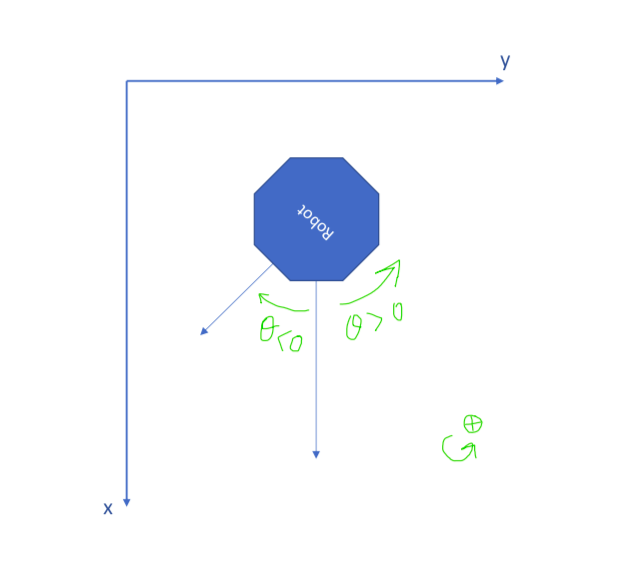
\includegraphics[scale=0.5]{theta}
\caption{Angle de repérage du robot}
\label{fig:theta}
\end{figure}

\subsection{Algorithme détaillé}

Dans le fichier main.py, la table de jeu est initialisée avec la disposition initiale des éléments, puis un timer est lancé pour arrêter le programme après 100 secondes qui est le temps limite du match fixé par le règlement de la coupe. On rentre ensuite dans une boucle while qui fait les actions suivantes:
\subsubsection{mettre à jour la table:}
Cette fonction commence par demander l'état de la caméra, si celle ci marche, tous les positions des éléments de la table sont mis à jour. \\ Dans le cas contraire, une solution d'urgence est nécessaire, en effet, puisque le robot ne voit plus la dispositions de tous les éléments de la table celui ci ne peut que se contenter de ce qu'il savait déjà de la table et de ce qu'il voit directement devant lui à travers les capteurs ceci lui permet de mettre à jour sa connaissance sur la table du jeu tout au long de son chemin vers la cible.

Dans ce cas, la fonction commence par mettre à jour la position et l'orientation de notre robot en se basant sur le retour de l'Arduino après avoir tenté d'accomplir la tache précédente, puis elle essaie de deviner les éléments que voit le robot à partir des données des capteurs et finit par mettre à jour les positions des éléments devinés.

Deviner un élément se fait de la manière suivante:
On commence par repérer tous les pairs de capteurs successifs qui permettent de deviner le centre d'un élément de diamètre d [le diamètre de l'atome ici], sachant que le robot contient six capteurs distribués uniformément sur le devant du robot et à 27° l'un de l'autre (la disposition optimale de n capteur devant le robot sera de les mettre uniformément espacées dans les 135° du devant figure \ref{fig:calcAngles}), ceci permet de deviner le centre de l'atome sachant la distance aux deux capteurs et le diamètre de l'atome (voir figure \ref{fig:calcDist}). 

\begin{figure}[!h]
\centering
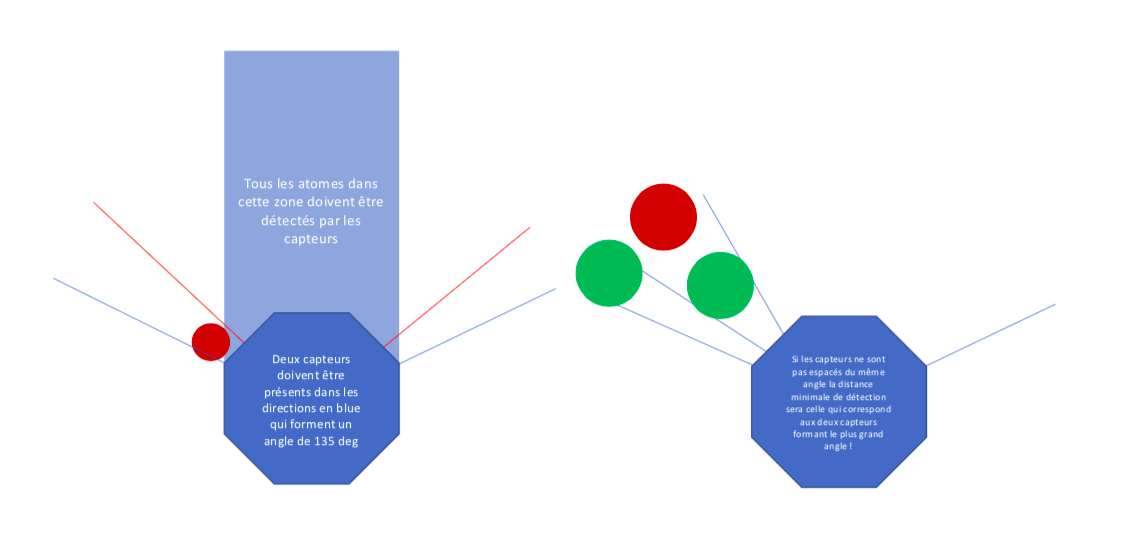
\includegraphics[scale=0.3]{calcAngles}
\caption{Positionnement optimal des capteurs pour éviter les zones mortes}
\label{fig:calcAngles}
\end{figure}

\begin{figure}[!h]
\centering
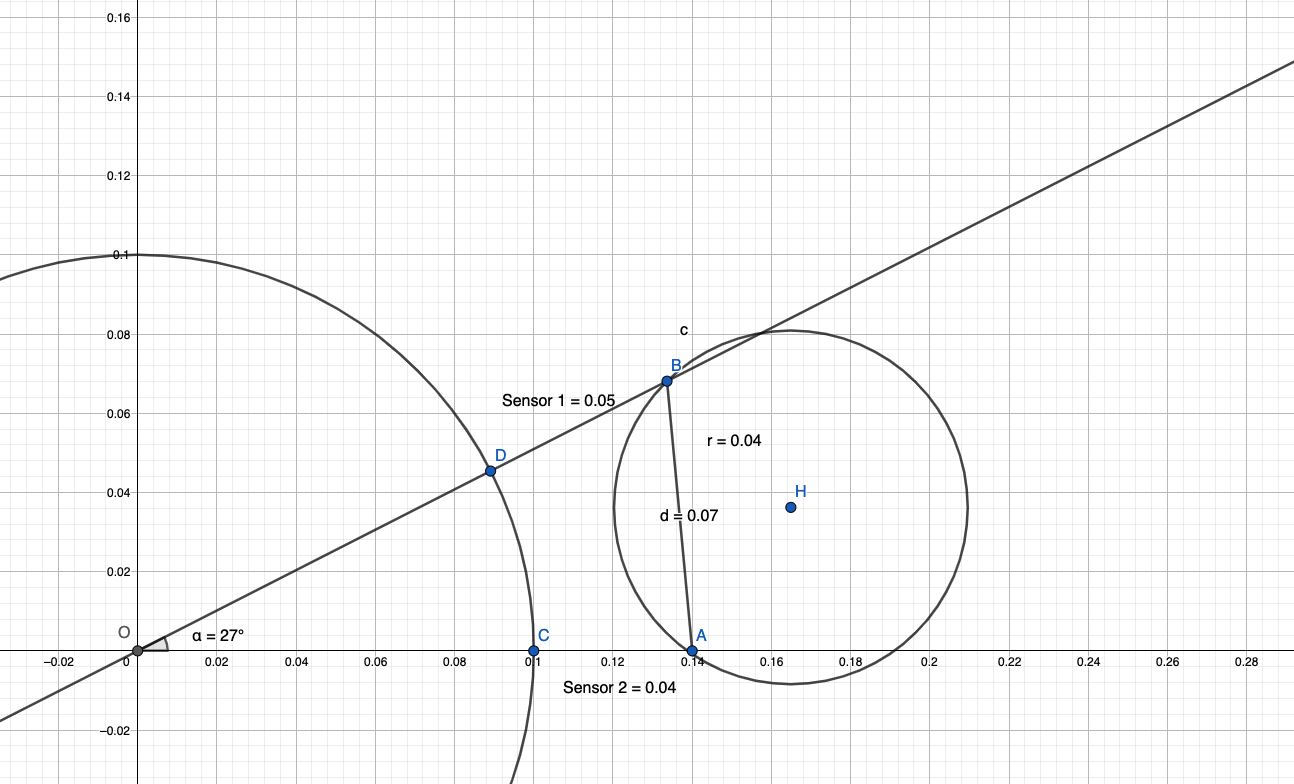
\includegraphics[scale=0.27]{calcDist}
\caption{Sachant les distances DB et CA et le diamètre de l'atome, le centre de l'atome peut être calculé}
\label{fig:calcDist}
\end{figure}

Vu que les cordonnées des points A et B sont connues dans la figure \ref{fig:calcDist} les distances aux capteurs doivent permettre d'avoir $d \leq 2r$, le calcul permet de trouver qu'avec six capteurs on peut trouver le centre d'un atome proche à 7 - 8 cm à peu près des deux capteurs (voir figure  \ref{fig:accZone}), ainsi on vérifie qu'on est bien dans la zone grise de la figure \ref{fig:accZone} avant de faire le calcul pour éviter les erreurs.

\begin{figure}[!h]
\centering
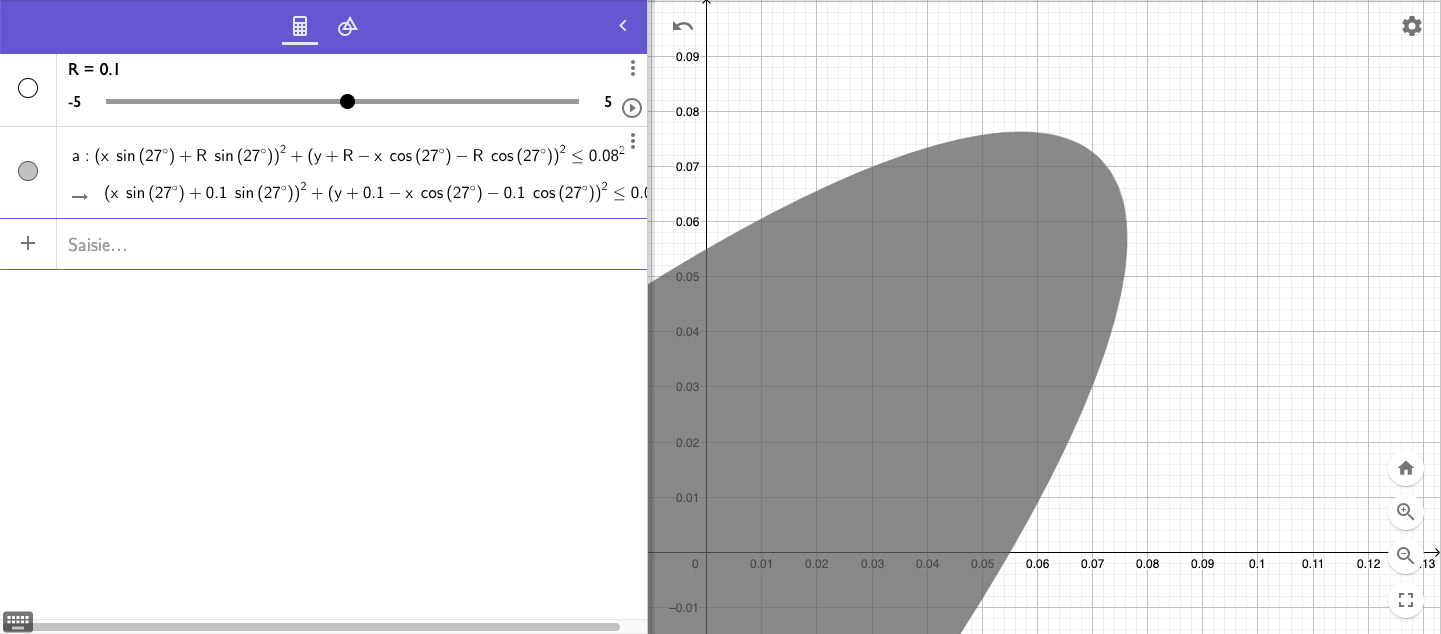
\includegraphics[scale=0.24]{accZone}
\caption{En gris les différentes pairs de distances (m) DB et CA qui vérifient la condition $d \leq 2r$ et permettent de calculer le centre de l'atome}
\label{fig:accZone}
\end{figure}

Il reste le cas où l'atome est sur les deux extrémités (c'est à dire qu'il est vu que par le capteur 0 tout seul ou le capteur 5 tout seul), dans ce cas on place l'atome en supposant que son centre est droit devant le capteur (c'est la solution la plus prudente).

Maintenant qu'on sait qu'il y a un atome à un point connu de la table (le centre calculé précédemment), il reste à choisir lequel des atomes doit on placer à cet endroit là, la solution choisie pour ce problème est d'y poser des atomes inutiles (dummy atoms). Remarquez que ce choix fait que si notre robot rencontre le robot adverse, celui ci le considère comme si c'était des atomes placés cote à cote devant le robot ce qui n'est pas un problème pour l'exécution de la suite des actions. Si il reste plus de dummy atoms, on reviens à la première et ainsi de suite. 
Si un atome inutile s'est fait bougé par le robot adverse ceci ne sera pas du tout un problème puisque ces atomes ne vont pas être utilisés dans des missions et par conséquence leurs positions exactes ne sont pas très importantes. Par contre s'il s'agit d'un atome principale ceci causera un problème et on aura plus la possibilité d'accomplir la mission correspondante ce qui est tout à fait normal car les capteurs seuls ne permettent pas de savoir ce qui se passe ailleurs d'où l'intérêt d'avoir le système de la caméra qui marche bien. En pratique ceci n'est pas un grand problème, en effet, le match ne dure pas très longtemps et dans la plupart des cas les robots s'occupent des atomes proches d'eux et n'aurons pas beaucoup d'influence sur le reste des atomes.


\subsubsection{envoyer l'action suivante:}

Étant donnée la nouvelle configuration de la table, cette fonction commence par tester si la mission en cours (stockée dans une variable globale currentMission) est encore faisable, si c'est pas le cas elle passe à la prochaine mission après avoir ordonné l'Arduino de poser l'atome si le robot porte une.

Après avoir trouver la mission à accomplir (i.e il existe un chemin vers la cible), on extrait du chemin trouvé sa première partie qui est une ligne droite. On aura ainsi l'angle initial que doit faire le robot pour se mettre sur cette droite et la longueur de ce premier segment du chemin, puis on demande au robot de tourner puis avancer pour faire cette première partie. L'idée est que le robot fait à chaque fois une rotation puis une translation continue jusqu'au prochain coin dans le chemin, cette idée est justifiée par le faire que le robot s'arrêtera en tout cas pour tourner ainsi le mieux c'est de lui demander de faire toute la partie droite avant le prochain virage.

Il est à noter que pour récupérer un atome le point cible pour calculer le chemin optimal doit être un des points au bord de la zone interdite au centre du robot (figure \ref{fig:zone}) et que le robot doit après son arriver à ce point ajuster son angle d'orientation pour pouvoir rattraper l'atome. Pour des raison de simplicité le point cible considéré est le plus proche point accessible sur le bord de la zone parmi les quatre points extrêmes suivant l'axe des abscisses et l'axe des ordonnées. (figure \ref{fig:pointsAcc})

\begin{figure}[!h]
\centering
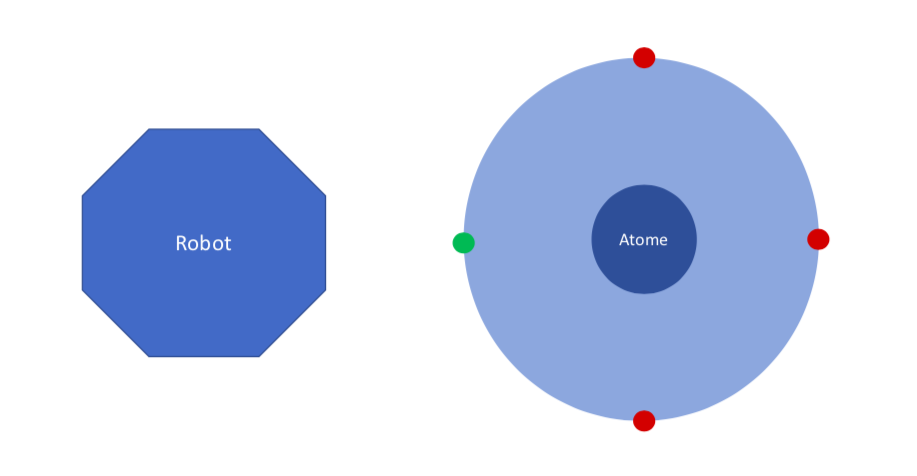
\includegraphics[scale=0.4]{pointAcc}
\caption{Le point cible qui sera considéré dans ce cas est le point en vert, c'est le point le plus proche au robot}
\label{fig:pointsAcc}
\end{figure}

Dans le cas où le robot arrive devant un atome, il l'a rattrape puis passe à la prochaine étape de la mission. Si le robot arrive à sa cible finale, il pose l'atome et augmente le score.


\subsection{Algorithme du plus court chemin}
L'algorithme de calcul du chemin optimal est implémenté dans le fichier \\   path\_finding\_algorithm.py, vous trouverez dedans (au moment de l'écriture de ces lignes) deux versions d'algorithmes codé dans les fonctions \textbf{astarV1(array, start, goal)} et \textbf{astarV2(array, start, goal)}, \textit{array} est une matrice où les zéros sont les cellules accessibles et les cellules contenant tout autre nombre représentent des obstacles, \textit{start} et \textit{goal} sont les deux tuples de cordonnées du point de départ et d'arrivée.

astarV1() implémente une version naïve de l'algorithme classique A* où les voisins de chaque point sont les huit voisins des cotés et des coins (les voisins de (0,0) par exemple sont [(0,1),(0,-1),(1,0),(-1,0),(1,1),(1,-1),(-1,1),(-1,-1)]), cet algorithme de type greedy visite les points en commençant par ceux qu'il pense être les points les plus proches à la destination (dans notre cas l'algorithme considère la distance euclidienne du point en cours à la cible), c'est un des algorithmes les plus classiques de calcul de chemins optimaux vu sa simplicité et sa faible consommation en mémoire. Voici un exemple de calcul de chemin entre deux points de la table en utilisant astarV1() (figure \ref{fig:astarV1})

Le problème dans cet implémentation naïve (et la motivation d'en trouver une amélioration) est le faite que celui-ci calcul des chemin certes optimales mais contenant beaucoup de virages (figure \ref{fig:astarV1}), sachant qu'à chaque itération de la boucle le robot reçoit un ordre de type \textit{tourner} puis \textit{avancer} et que faire tourner le robot consomme du temps, l'algorithme précèdent est loin d'être optimale si le chemin est évalué en terme de durée de parcours, l'idée est alors de trouver une amélioration de A* où les chemins contiennent le moins de virages possibles sans perdre de l'optimalité spatiale de l'algorithme, étant donné que le souci ici est de réaliser les taches le plus rapidement possible.

\begin{figure}[!h]
\centering
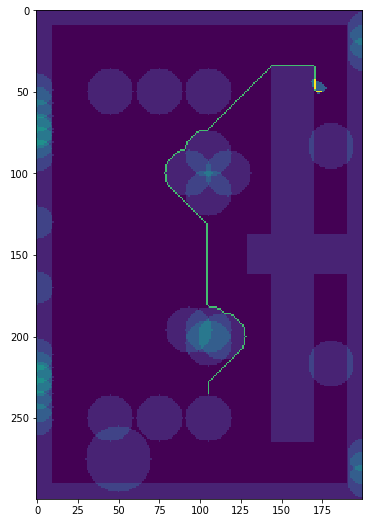
\includegraphics[scale=0.6]{astarV1}
\caption{Calcul de chemin optimal en utilisant l'algorithme A* naïf}
\label{fig:astarV1}
\end{figure}

L'idée implémentée dans le astarV2() est la suivante:
Étant donné deux points A et B de la table, au lieu permettre à l'algorithme de parcourir toute la table pour trouver un chemin, on commence par des résolution plus faibles et on augmente la résolution jusqu'à ce qu'on trouve le chemin, par exemple, dans la figure \ref{fig:resol}, on a commencé par chercher le chemin entre A et B avec une résolution $res_{x} = |A_{x}-B_{x}|$ en x et $res_{y} = |A_{y}-B_{y}|$ en y où $A_{x}, A_{y}$ et $B_{x}, B_{y}$ représentent les cordonnées du point A et B respectivement dans la matrice, ce qui veut dire que seuls les points de la table qui s'écrivent comme $(A_{x} + n \times res_{x}, A_{y} + m \times res_{y})$ vont être parcourus par l'algorithme (dans le cas où l'un de ces deux résolutions et nul on lui donne 1), si un tel chemin existe celui-ci contiendra très peu de virages et sera ainsi plus rapide à parcourir, dans le cas contraire on augmente la résolution en choisissant de façon décroissante $res_{x}$ dans l'ensemble des diviseurs de $|A_{x}-B_{x}|$ et $res_{y}$ dans l'ensemble des diviseurs de $|A_{y}-B_{y}|$ (pour s'assurer que la grille $\{A_{x} + n \times res_{x}, A_{y} + m \times res_{y}\}_{n \in Z, m \in Z} \bigcap \{(x, y)\}_{(x,y) \in table}$ contient le point cible B) (voir figure \ref{fig:grille})

\begin{figure}[!h]
\centering
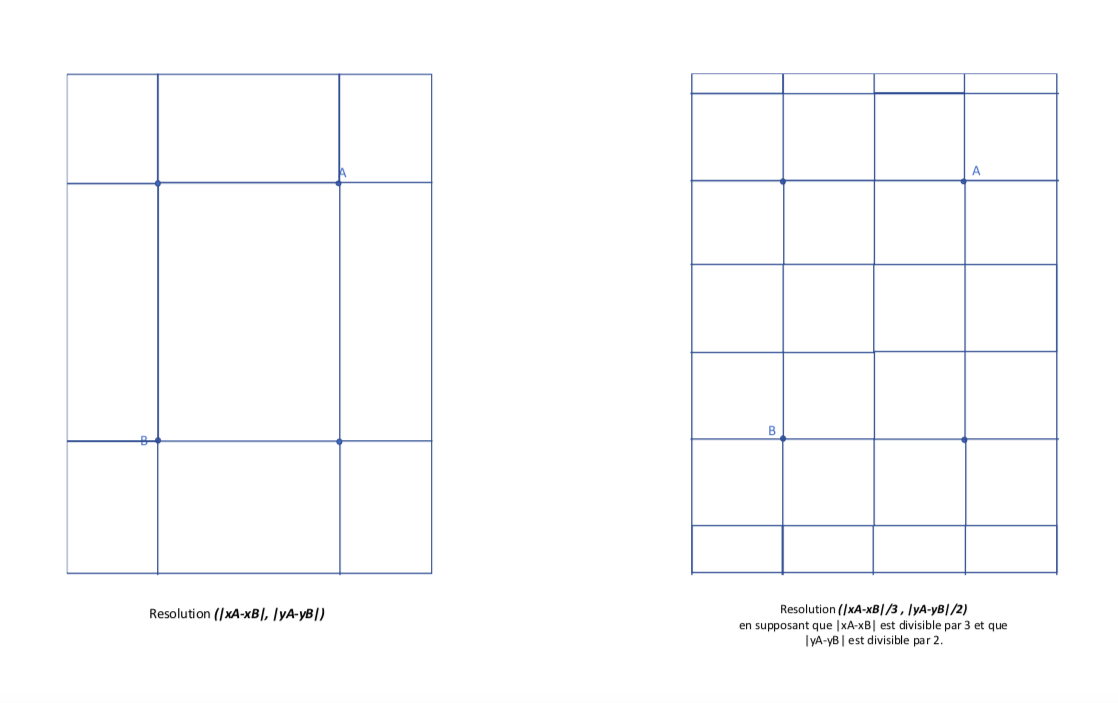
\includegraphics[scale=0.3]{resol}
\caption{Implémentation de l'idée des résolutions}
\label{fig:resol}
\end{figure}

\begin{figure}[!h]
\centering
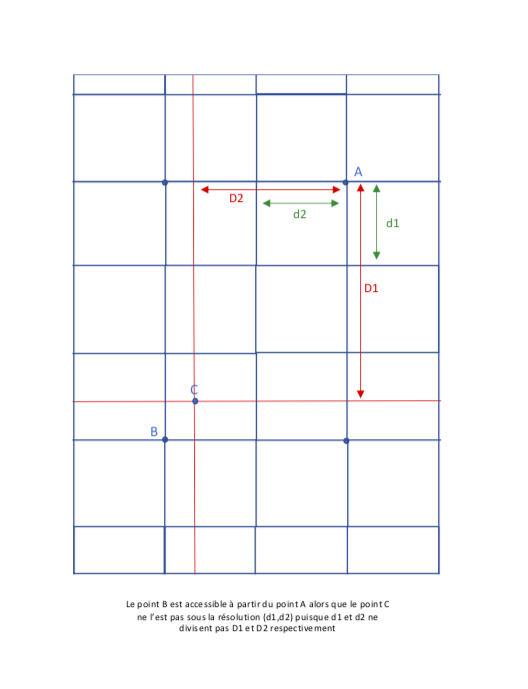
\includegraphics[scale=0.6]{grille}
\caption{Points accessibles sous une résolution donnée}
\label{fig:grille}
\end{figure}

Pour mettre en place cette idée il suffit de modifier l'ensemble des voisins d'un élément dans l'algorithme naif, en effet, les voisins d'un élément $(x,y)$ sous la résolution $res_{x}, res_{y}$ seront cette fois ci $\{(a,b) \in \{(x+res_{x}, y), (x-res_{x}, y), (x, y + res_{y}), (x, y - res_{y})\}$ tels que $table[i][j] = 0$ pour $i \in (a,x)$ et $j \in (b,y)\}$ , c'est à dire les éléments voisins (avec la résolution considérée) qui sont accessibles en ligne droite depuis le point de départ (x,y). Si le chemin n'a pas été trouvé, on augmente la résolution en passant à de plus petit diviseurs et donc des voisins plus proches. Ceci veut dire que l'algorithme converge et on tombera dans le pire des cas sur la résolution (1,1) qui est rien que l'algorithme naïf astarV1().  

Les nouveaux chemin sont maintenant plus rapide à calculer (le chemin peut être trouvé sans avoir besoin de passer à une grade résolution) et ont moins de virages (figure \ref{fig:astarV2})

\begin{figure}[!h]
\centering
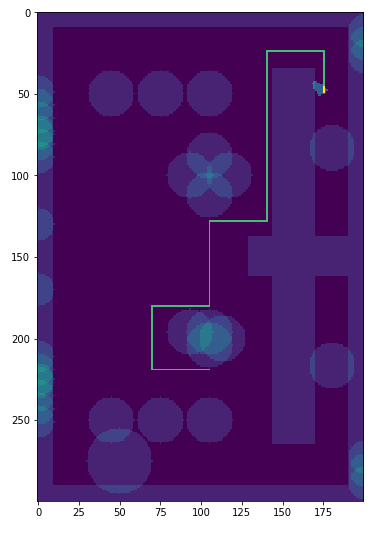
\includegraphics[scale=0.6]{astarV2}
\caption{Calcul de chemin optimal en utilisant l'algorithme A* optimisé}
\label{fig:astarV2}
\end{figure}

\subsection{Tests}
\subsubsection{Construction de la table}
Comme mentionné précédemment, la table du jeu est initialisée à une matrice de zéros, ensuite, les obstacles statiques de la table sont ajoutés et enfin on ajoute toutes les zones correspondantes à la disposition initiale des atomes. Les tests 1, 2, 3 et 4 permettent de tester cela. (figure \ref{fig:tests1})

\begin{figure}[!h]
\centering
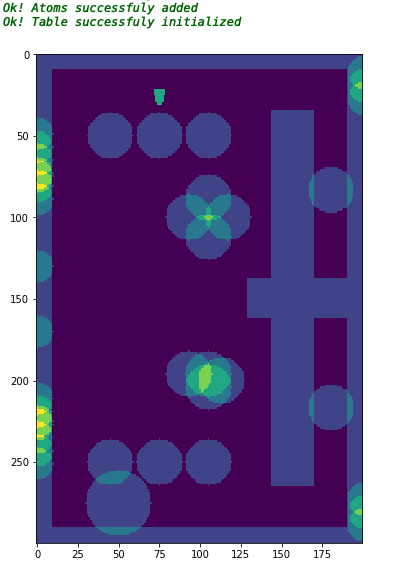
\includegraphics[scale=0.6]{tests1}
\caption{Construction et ajout des differents elements de la table}
\label{fig:tests1}
\end{figure}

\subsubsection{calcul de chemin}
Le test 5 et 6 permettent de calculer et dessiner le chemin optimal entre le robot et un atome de la table (pour passer de \textit{astarV2()} à \textit{astarV1()} changer le retour de la fonction \textit{algorithme()} dans le fichier \textit{path\_finding\_algorithm.py}) (figure \ref{fig:tests2})

\begin{figure}[!h]
\centering
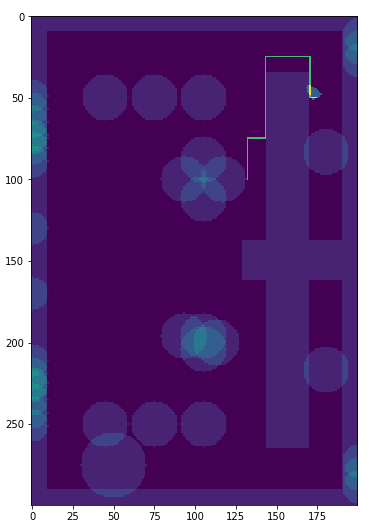
\includegraphics[scale=0.6]{tests2}
\caption{Calcul du chemin optimale à une atome de la table}
\label{fig:tests2}
\end{figure}

\subsubsection{fonctions utiles}

La fonction \textit{getThetaFromSourceToTarget()} du \textit{test7()} permet de calculer l'angle entre une source et une cible avec la convention de la figure \ref{fig:theta}.

Dans le \textit{test8()} et \textit{test9()},  \textit{updateOurRobotPosition()} et \textit{updatePosition()} permettent de mettre à jour la position de notre robot et d'un élément quelconque de la table respectivement.

Ensuite le \textit{test10()}, \textit{test11()} testent les fonctions \textit{getExpXY()} et \textit{theRobotIsLookingAt()} qui calculent respectivement le centre d'un élément à deux distances données des capteurs et prédisent l'élément à partir d'une réponse de l'Arduino

Finalement, \textit{updateTable()} dans le \textit{test12()} est une des deux fonctions principales du programme (avec la fonction \textit{sendNextAction()}) qui permet de mettre à jour la table à partir d'une réponse de l'Arduino (et de la caméra au cas où celle ci marche bien)

Pour tester l'ensemble de l'algorithme \textit{mn.action()} fait appel à la boucle principale qui lance le programme, vous verrez le robot qui est entrain de calculer son chemin, envoyer les consignes à \textit{connect\_robot.py}, qui lui rendra une réponse puis une mise à jour de la table est fait où vous verrez que le robot a fait une rotation et le premier segment du chemin, le cycle recommence tant que la mission est faisable, dans le cas contraire le robot passe à la mission suivante. (\ref{fig:tests3})

\begin{figure}[!h]
\centering
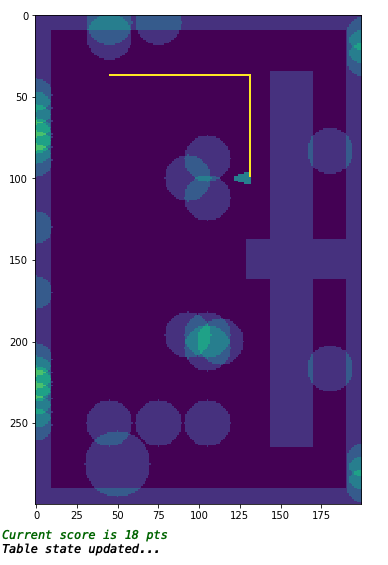
\includegraphics[scale=0.6]{tests3}
\caption{L'algorithme en action}
\label{fig:tests3}
\end{figure}

Finalement pour simuler un obstacle devant le robot, on doit jouer sur la réponse de l'Arduino, celle ci est codée dans le fichier \textit{connect\_robot.py} de façon à ce qu'elle envoie que le mission était bien accomplie et que le robot a bien fait la distance ou l'angle qui lui a été demandé. Pour simuler un obstacle, vous pouvez dé-commenter la partie correspondante (voir l'explication en haut du fichier \textit{connect\_robot.py}) et vous verrez que le robot s'arrête devant l'obstacle et calculera un nouveau chemin comme prévu (figure \ref{fig:obstacle}).

\begin{figure}[!h]
\centering
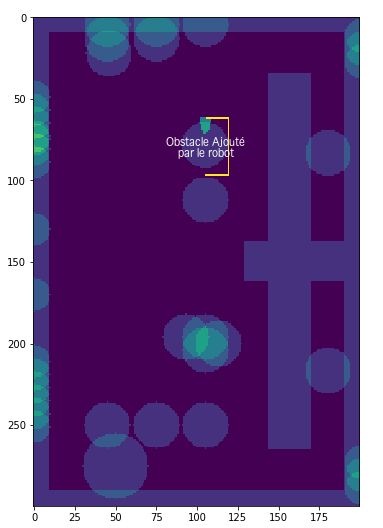
\includegraphics[scale=0.6]{obstacle}
\caption{Ajout d'un obstacle par le robot et recalcule du nouveau chemin optimal}
\label{fig:obstacle}
\end{figure}

\section{Point sur le travail fait par le group mécanique:}

\bibliographystyle{plain}
\bibliography{references}
\end{document}
